%%%%%%%%%%%%%%%%%%%%%%%%%%%%%%%%%%%%%%%%%
% Beamer Presentation
% LaTeX Template
% Version 1.0 (10/11/12)
%
% This template has been downloaded from:
% http://www.LaTeXTemplates.com
%
% License:
% CC BY-NC-SA 3.0 (http://creativecommons.org/licenses/by-nc-sa/3.0/)
%
%%%%%%%%%%%%%%%%%%%%%%%%%%%%%%%%%%%%%%%%%

%----------------------------------------------------------------------------------------
%	PACKAGES AND THEMES
%----------------------------------------------------------------------------------------

\documentclass{beamer}

\mode<presentation> {

% The Beamer class comes with a number of default slide themes
% which change the colors and layouts of slides. Below this is a list
% of all the themes, uncomment each in turn to see what they look like.

%\usetheme{default}
%\usetheme{AnnArbor}
%\usetheme{Antibes}
%\usetheme{Bergen}
%\usetheme{Berkeley}
%\usetheme{Berlin}
%\usetheme{Boadilla}
%\usetheme{CambridgeUS}
%\usetheme{Copenhagen}
%\usetheme{Darmstadt}
%\usetheme{Dresden}
%\usetheme{Frankfurt}
%\usetheme{Goettingen}
%\usetheme{Hannover}
%\usetheme{Ilmenau}
%\usetheme{JuanLesPins}
%\usetheme{Luebeck}
\usetheme{Madrid}
%\usetheme{Malmoe}
%\usetheme{Marburg}
%\usetheme{Montpellier}
%\usetheme{PaloAlto}
%\usetheme{Pittsburgh}
%\usetheme{Rochester}
%\usetheme{Singapore}
%\usetheme{Szeged}
%\usetheme{Warsaw}

% As well as themes, the Beamer class has a number of color themes
% for any slide theme. Uncomment each of these in turn to see how it
% changes the colors of your current slide theme.

%\usecolortheme{albatross}
%\usecolortheme{beaver}
%\usecolortheme{beetle}
%\usecolortheme{crane}
%\usecolortheme{dolphin}
%\usecolortheme{dove}
%\usecolortheme{fly}
%\usecolortheme{lily}
%\usecolortheme{orchid}
%\usecolortheme{rose}
%\usecolortheme{seagull}
%\usecolortheme{seahorse}
%\usecolortheme{whale}
%\usecolortheme{wolverine}

%\setbeamertemplate{footline} % To remove the footer line in all slides uncomment this line
%\setbeamertemplate{footline}[page number] % To replace the footer line in all slides with a simple slide count uncomment this line

%\setbeamertemplate{navigation symbols}{} % To remove the navigation symbols from the bottom of all slides uncomment this line
}

\usepackage{graphicx} % Allows including images
\usepackage{booktabs} % Allows the use of \toprule, \midrule and \bottomrule in tables
\usepackage{multirow}
\usepackage{xcolor}
\newcommand{\xmark}{\textcolor{red}{\text{\sffamily X}}}
\newcommand{\cmark}{\textcolor{green}{\checkmark}}
\newcommand{\tr}{\text{tr}}
\newcommand{\E}{\textbf{E}}
\newcommand{\diag}{\text{diag}}
\newcommand{\argmax}{\text{argmax}}
\newcommand{\argmin}{\text{argmin}}
\newcommand{\Cov}{\text{Cov}}
\newcommand{\Vol}{\text{Vol}}
\newcommand{\blue[1]}{\color{blue}{\textbf{#1}}}

%----------------------------------------------------------------------------------------
%	TITLE PAGE
%----------------------------------------------------------------------------------------


\title{All-Pairs-Shortest-Paths in Spark}

\author{Charles Zheng, Jingshu Wang and Arzav Jain} % Your name
\institute[Stanford] % Your institution as it will appear on the bottom of every slide, may be shorthand to save space
{Stanford University}
\date{\today} % Date, can be changed to a custom date

\begin{document}

\begin{frame}
\titlepage % Print the title page as the first slide
\end{frame}

\section{Introduction}

\begin{frame}
\frametitle{Problem}
\begin{itemize}
\item Weighted graph $G = (V, E)$ with $n$ vertices
\item Compute $n \times n$ matrix of distances $S$ where
\[
S_{ij} = \text{weight of shortest path from $i$ to $j$}
\]
\begin{center}
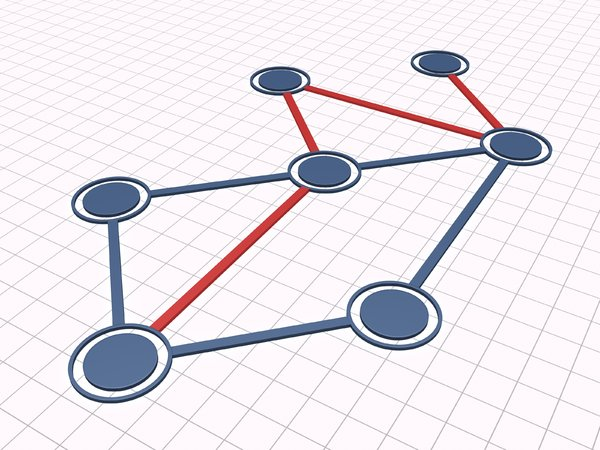
\includegraphics[scale = 0.3]{stock_sp.jpg}
\end{center}
\end{itemize}
\end{frame}

\begin{frame}
\frametitle{Floyd-Warshall}
Initial input
\begin{tabular}{cc}
$
\begin{pmatrix}
0&1& & & &1\\
1&0&1& & & \\
 &1&0&1& & \\
 & &1&0&1& \\
 & & &1&0&1\\
1& & & &1&0\\
\end{pmatrix}
$
&
\raisebox{-.5\height}{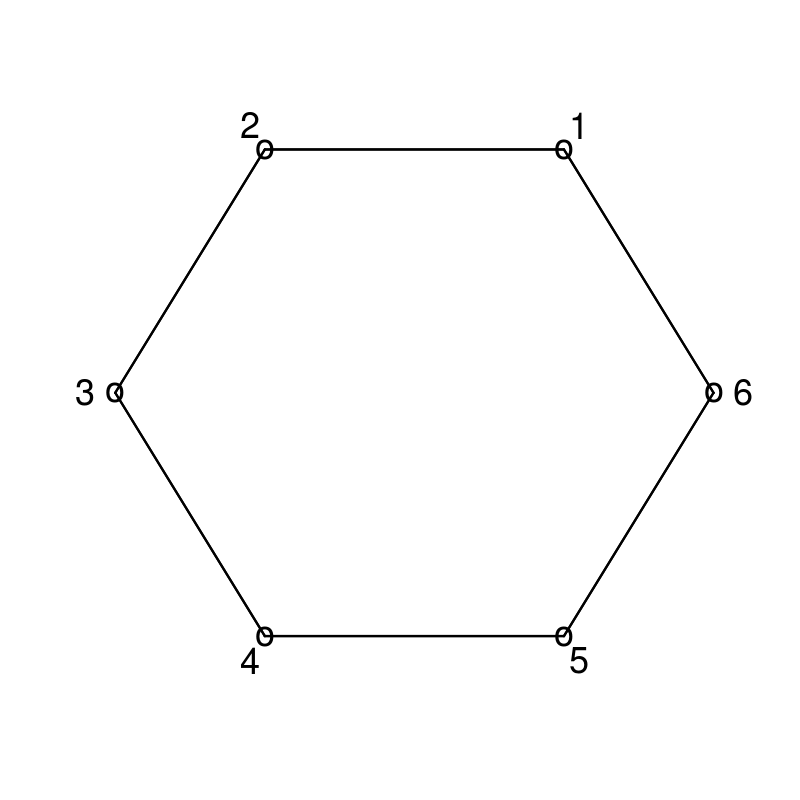
\includegraphics[scale = 0.3]{../figures/fig1_00.png}}
\end{tabular}
\end{frame}

\begin{frame}
\frametitle{Floyd-Warshall}
Iteration 1
\begin{tabular}{cc}
$
\begin{pmatrix}
0&1& & & &1\\
1&0&1& & &\blue[2]\\
 &1&0&1& & \\
 & &1&0&1& \\
 & & &1&0&1\\
1&\blue[2]& & &1&0\\
\end{pmatrix}
$
&
\raisebox{-.5\height}{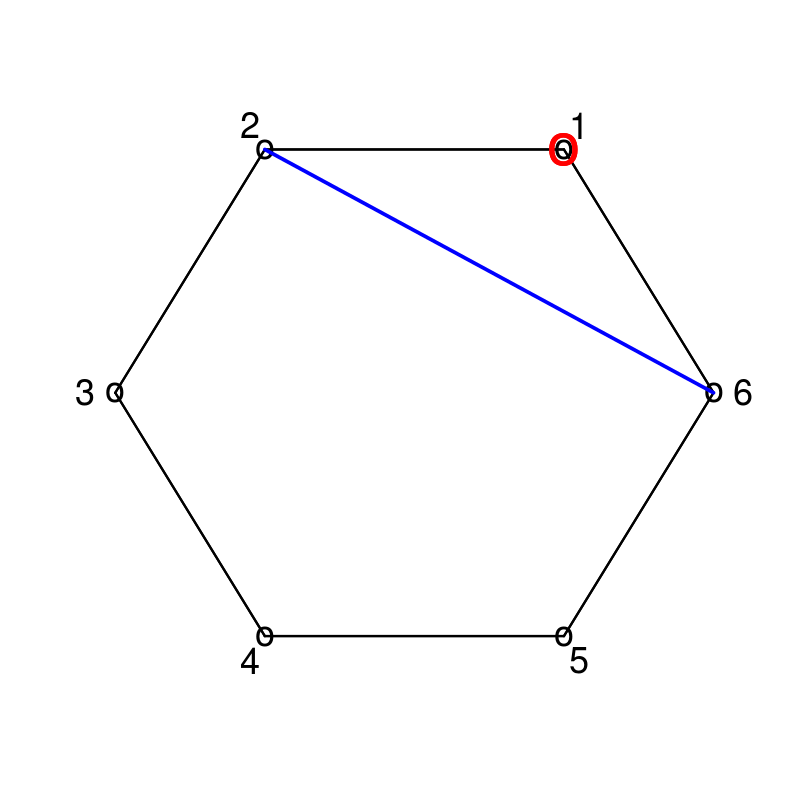
\includegraphics[scale = 0.3]{../figures/fig1_01.png}}
\end{tabular}
\end{frame}

\begin{frame}
\frametitle{Floyd-Warshall}
Iteration 2
\begin{tabular}{cc}
$
\begin{pmatrix}
0&1&\blue[2]& & &1\\
1&0&1& & &2\\
\blue[2]&1&0&1& &\blue[3]\\
 & &1&0&1& \\
 & & &1&0&1\\
1&2&\blue[3]& &1&0\\
\end{pmatrix}
$
&
\raisebox{-.5\height}{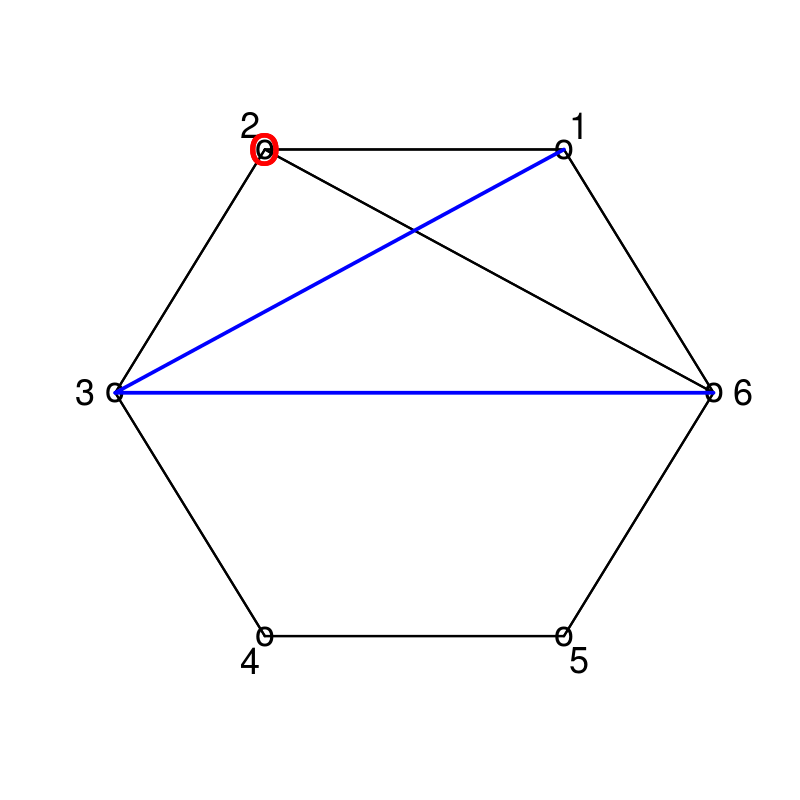
\includegraphics[scale = 0.3]{../figures/fig1_02.png}}
\end{tabular}
\end{frame}

\begin{frame}
\frametitle{Floyd-Warshall}
Iteration 3
\begin{tabular}{cc}
$
\begin{pmatrix}
0&1&2&\blue[3]& &1\\
1&0&1&\blue[2]& &2\\
2&1&0&1& &3\\
\blue[3]&\blue[2]&1&0&1&\blue[4]\\
 & & &1&0&1\\
1&2&3&\blue[4]&1&0\\
\end{pmatrix}
$
&
\raisebox{-.5\height}{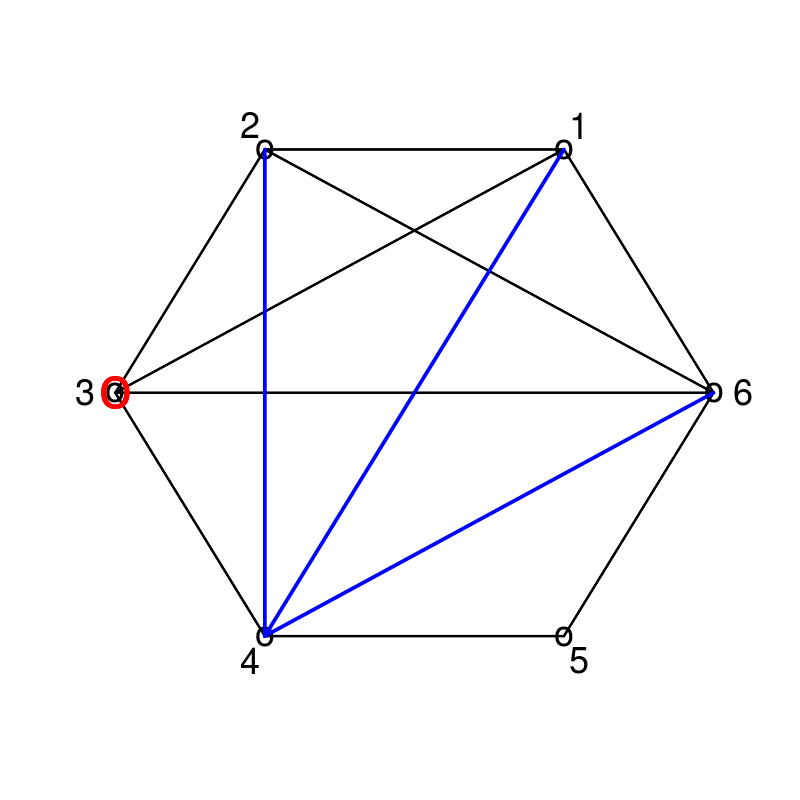
\includegraphics[scale = 0.3]{../figures/fig1_03.png}}
\end{tabular}
\end{frame}


\begin{frame}
\frametitle{Floyd-Warshall}
Iteration 4
\begin{tabular}{cc}
$
\begin{pmatrix}
0&1&2&3&\blue[4]&1\\
1&0&1&2&\blue[3]&2\\
2&1&0&1&\blue[2]&3\\
3&2&1&0&1&4\\
\blue[4]&\blue[3]&\blue[2]&1&0&1\\
1&2&3&4&1&0\\
\end{pmatrix}
$
&
\raisebox{-.5\height}{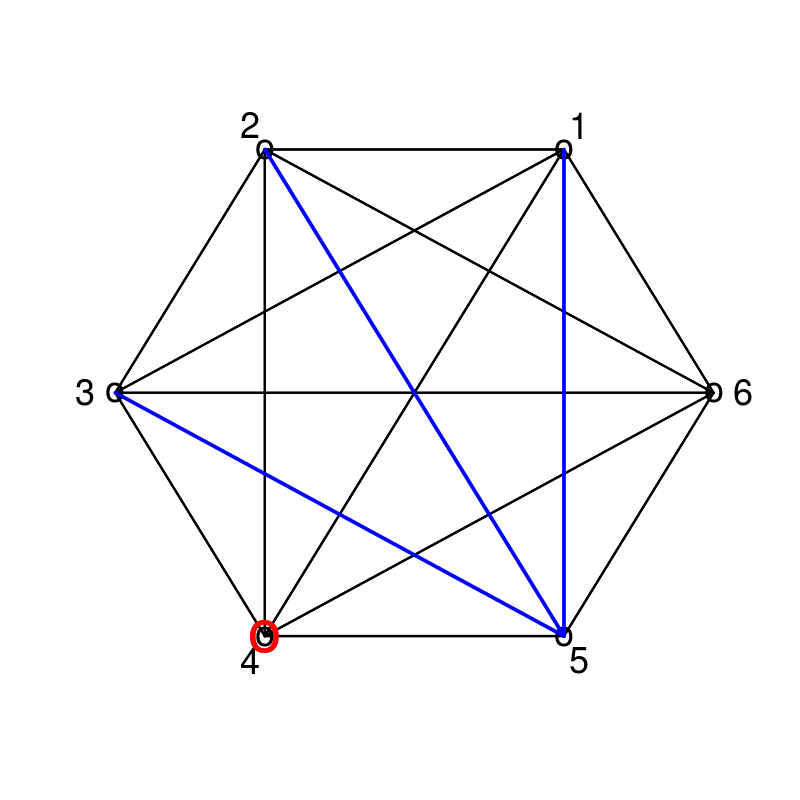
\includegraphics[scale = 0.3]{../figures/fig1_04.png}}
\end{tabular}
\end{frame}

\begin{frame}
\frametitle{Floyd-Warshall}
Iteration 5
\begin{tabular}{cc}
$
\begin{pmatrix}
0&1&2&3&4&1\\
1&0&1&2&3&2\\
2&1&0&1&2&3\\
3&2&1&0&1&\blue[2]\\
4&3&2&1&0&1\\
1&2&3&\blue[2]&1&0\\
\end{pmatrix}
$
&
\raisebox{-.5\height}{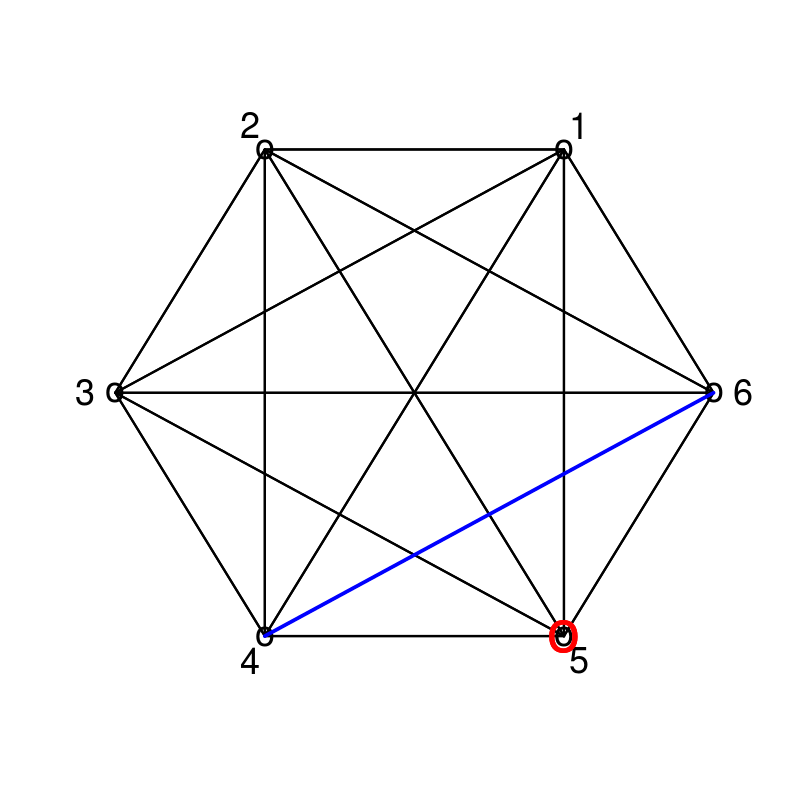
\includegraphics[scale = 0.3]{../figures/fig1_05.png}}
\end{tabular}
\end{frame}

\begin{frame}
\frametitle{Floyd-Warshall}
Iteration 6, \emph{(terminate)}
\begin{tabular}{cc}
$
\begin{pmatrix}
0&1&2&3&\blue[2]&1\\
1&0&1&2&3&2\\
2&1&0&1&2&3\\
3&2&1&0&1&2\\
\blue[2]&3&2&1&0&1\\
1&2&3&2&1&0\\
\end{pmatrix}
$
&
\raisebox{-.5\height}{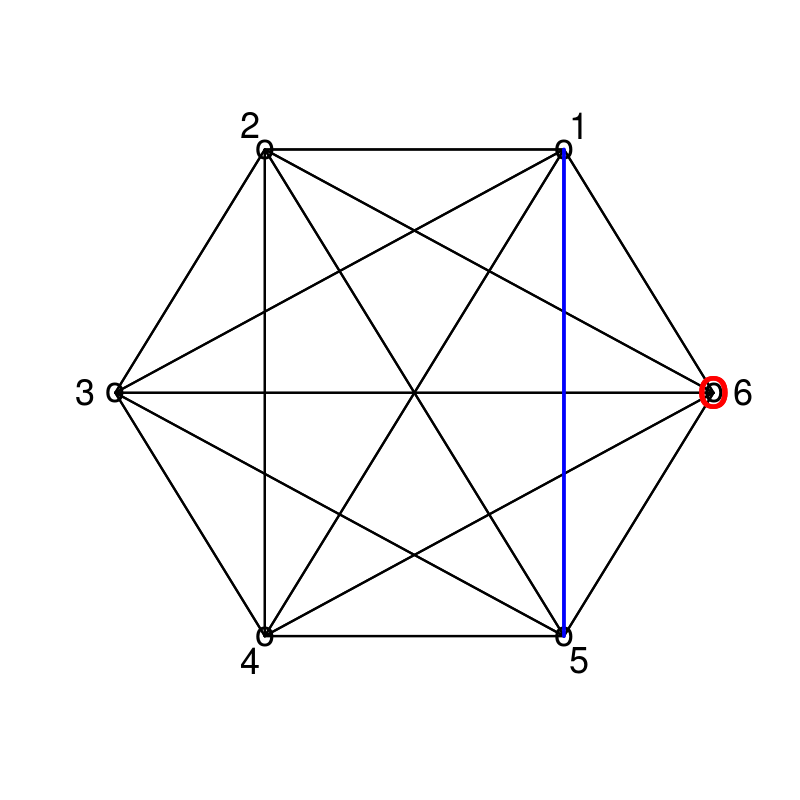
\includegraphics[scale = 0.3]{../figures/fig1_06.png}}
\end{tabular}
\end{frame}

\begin{frame}
\frametitle{Floyd-Warshall}
\begin{itemize}
\item Cost: $O(n^3)$ operations (single-core)
\item Takes $n$ \emph{sequential} iterations
\end{itemize}

\end{frame}

\begin{frame}
\frametitle{Problems with Floyd-Warshall}
\begin{itemize}
\item FW updates using 1 vertex at a time
\item Result: $n$ iterations
\item High \# iterations = \emph{latency} in distributed setting
\item Solomonik et al. (2013) show how to ``block'' FW iterates
\item We modify their block-based approach for Spark
\end{itemize}
\end{frame}

\begin{frame}
\frametitle{Block APSP}
Initial input: $n = 24$, \emph{block size} = $8$
\begin{tabular}{cc}
\raisebox{-.5\height}{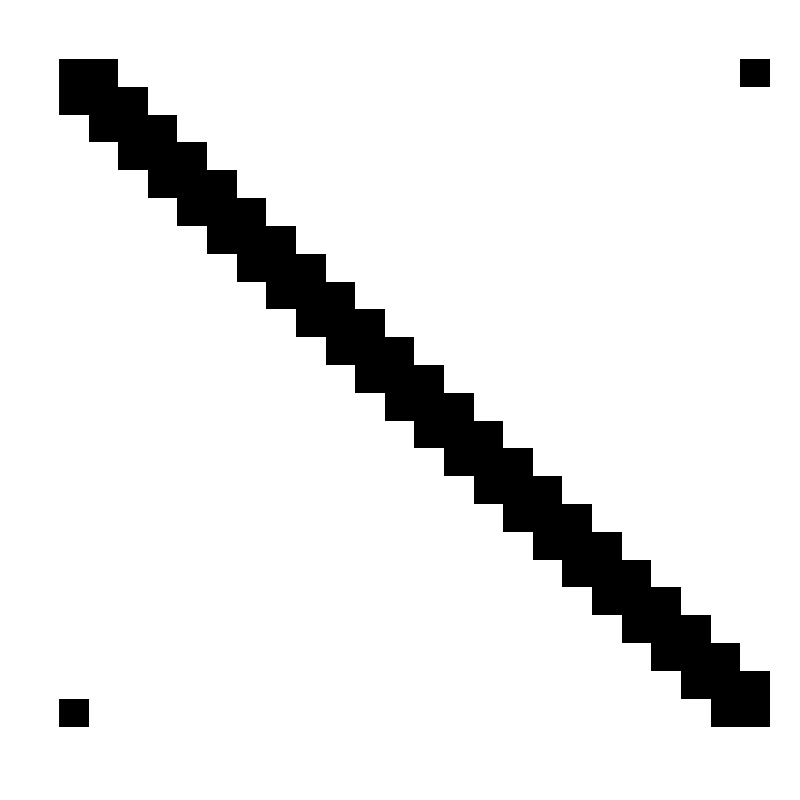
\includegraphics[scale = 0.1]{../figures/fig2_00m.png}}
&
\raisebox{-.5\height}{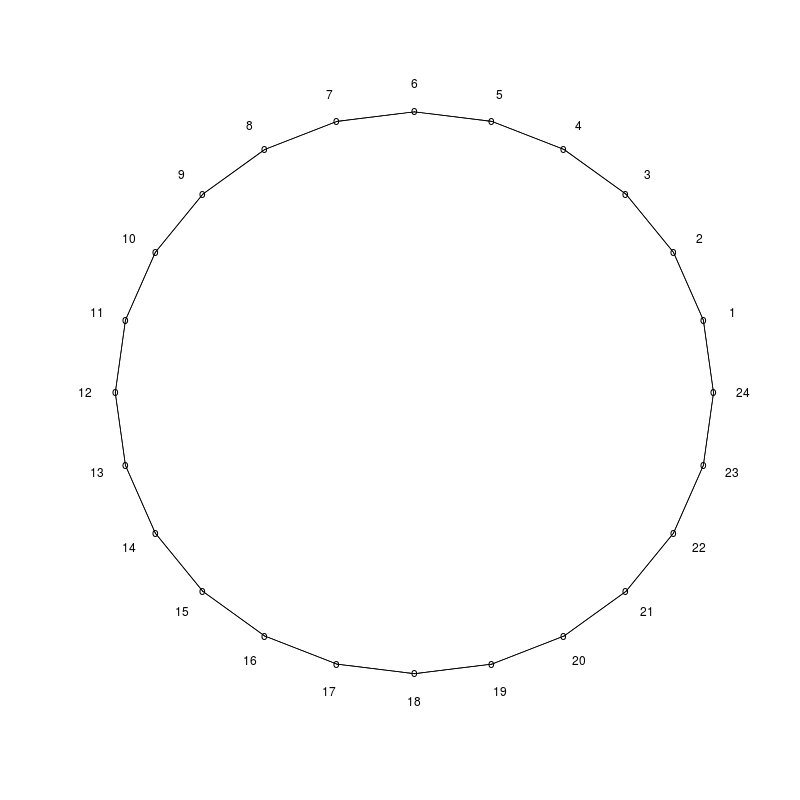
\includegraphics[scale = 0.3]{../figures/fig2_00.png}}
\end{tabular}
\end{frame}

\begin{frame}
\frametitle{Block APSP}
Iteration 1A: Update all paths within block 1 (with FW)
\begin{tabular}{cc}
\raisebox{-.5\height}{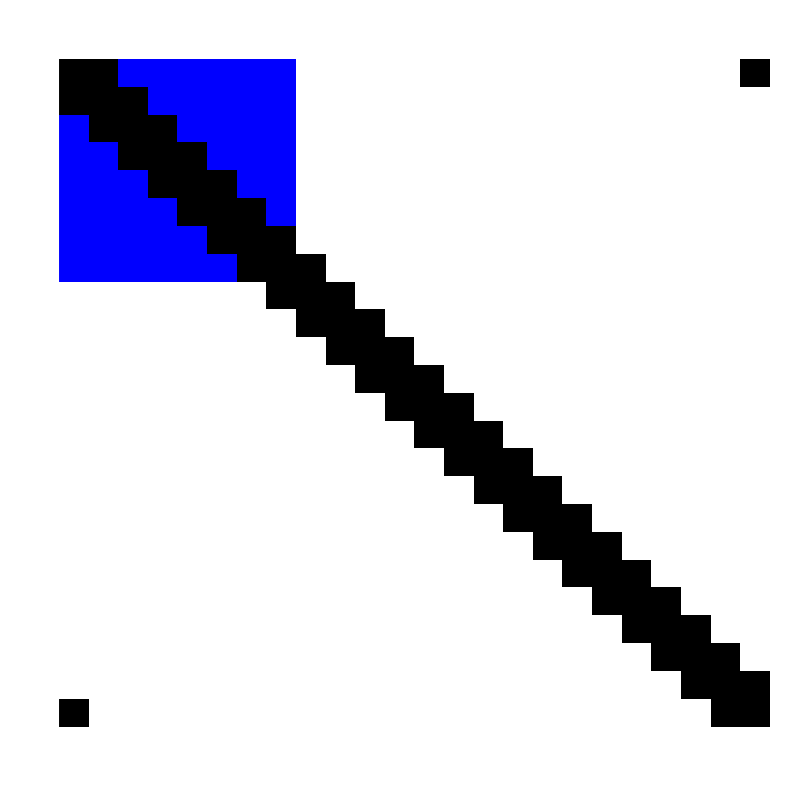
\includegraphics[scale = 0.1]{../figures/fig2_01am.png}}
&
\raisebox{-.5\height}{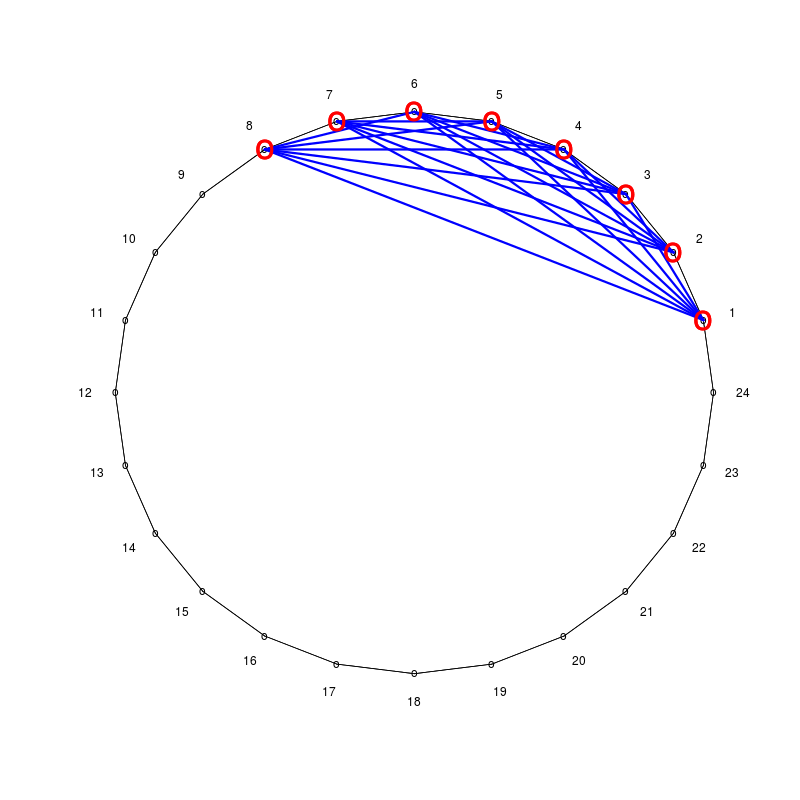
\includegraphics[scale = 0.3]{../figures/fig2_01a.png}}
\end{tabular}
\end{frame}

\begin{frame}
\frametitle{Block APSP}
Iteration 1B: Update all paths to/from block 1
\begin{tabular}{cc}
\raisebox{-.5\height}{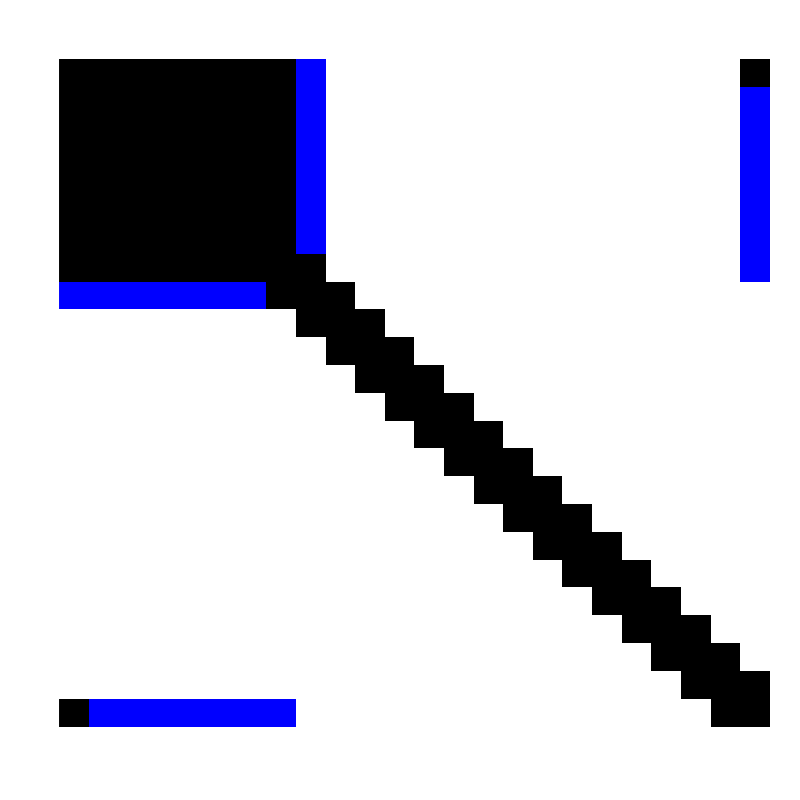
\includegraphics[scale = 0.1]{../figures/fig2_01bm.png}}
&
\raisebox{-.5\height}{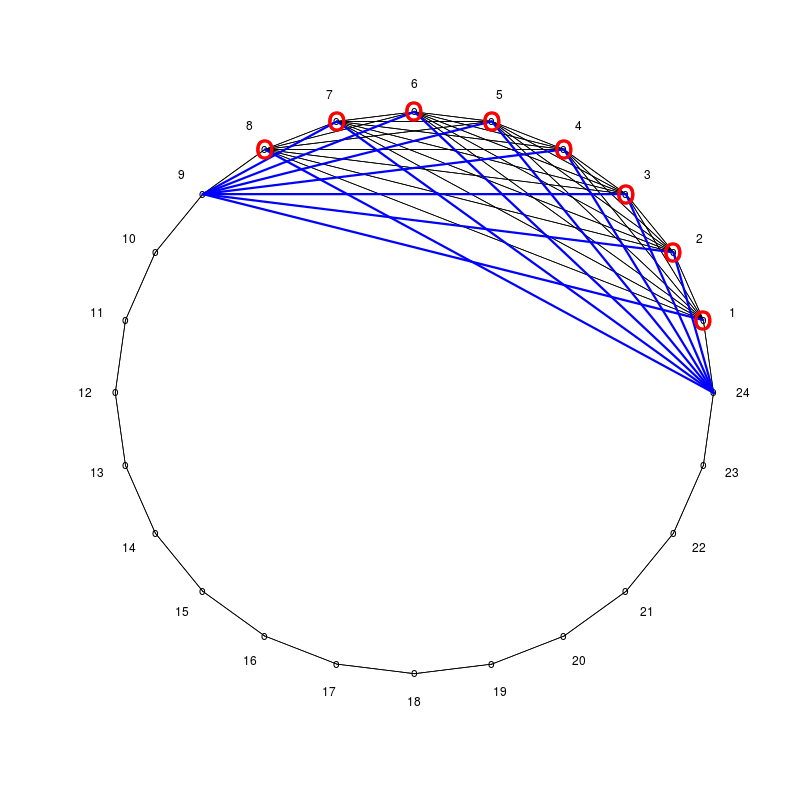
\includegraphics[scale = 0.3]{../figures/fig2_01b.png}}
\end{tabular}
\end{frame}

\begin{frame}
\frametitle{Block APSP}
Iteration 1C: Update all paths
\begin{tabular}{cc}
\raisebox{-.5\height}{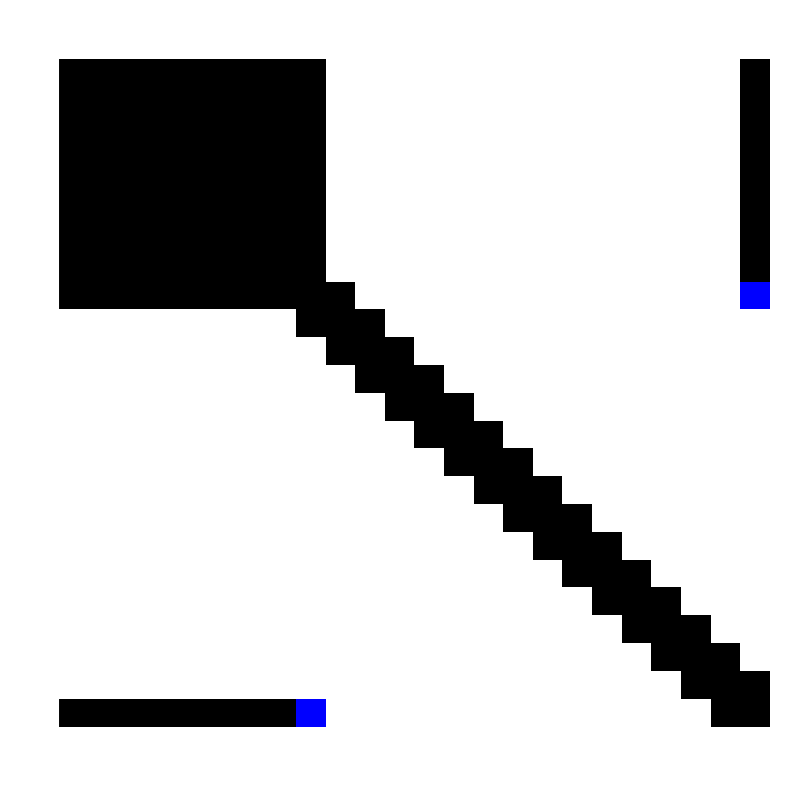
\includegraphics[scale = 0.1]{../figures/fig2_01cm.png}}
&
\raisebox{-.5\height}{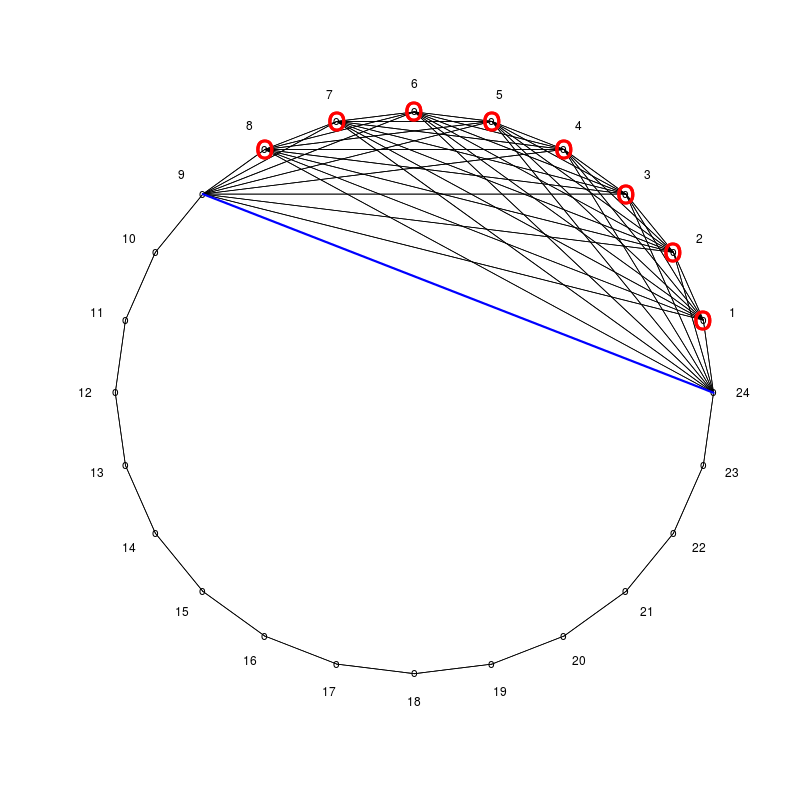
\includegraphics[scale = 0.3]{../figures/fig2_01c.png}}
\end{tabular}
\end{frame}


\begin{frame}
\frametitle{Block APSP}
Iteration 2A: Update all paths within block 2 (with FW)
\begin{tabular}{cc}
\raisebox{-.5\height}{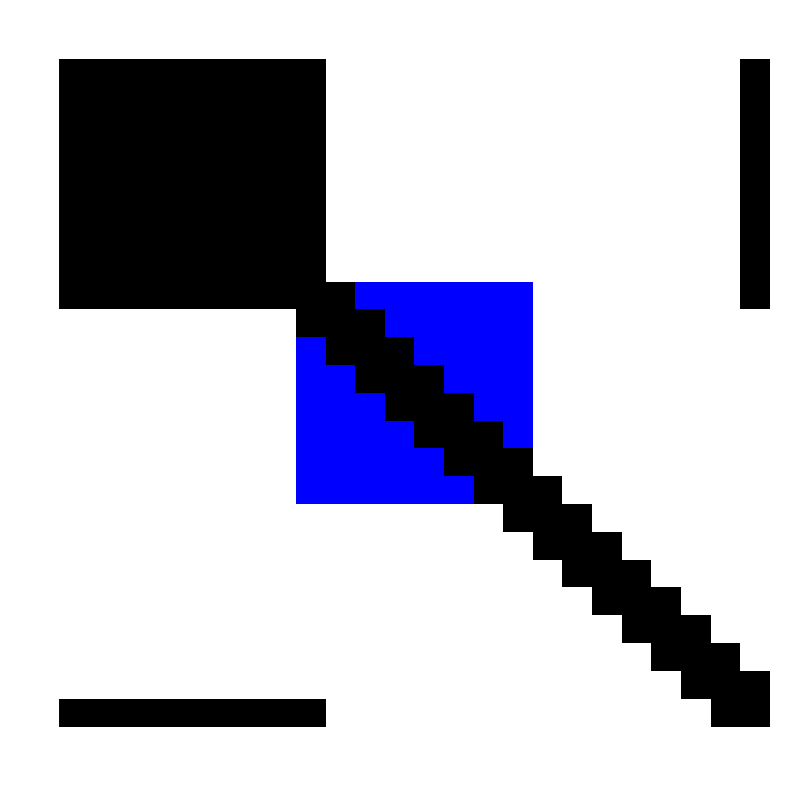
\includegraphics[scale = 0.1]{../figures/fig2_02am.png}}
&
\raisebox{-.5\height}{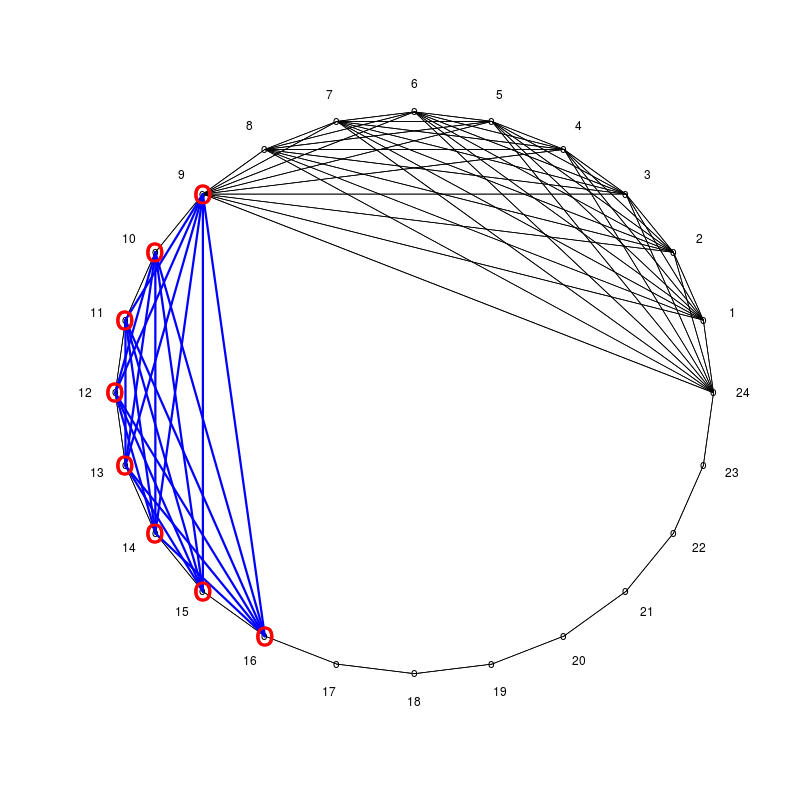
\includegraphics[scale = 0.3]{../figures/fig2_02a.png}}
\end{tabular}
\end{frame}

\begin{frame}
\frametitle{Block APSP}
Iteration 2B: Update all paths to/from block 2
\begin{tabular}{cc}
\raisebox{-.5\height}{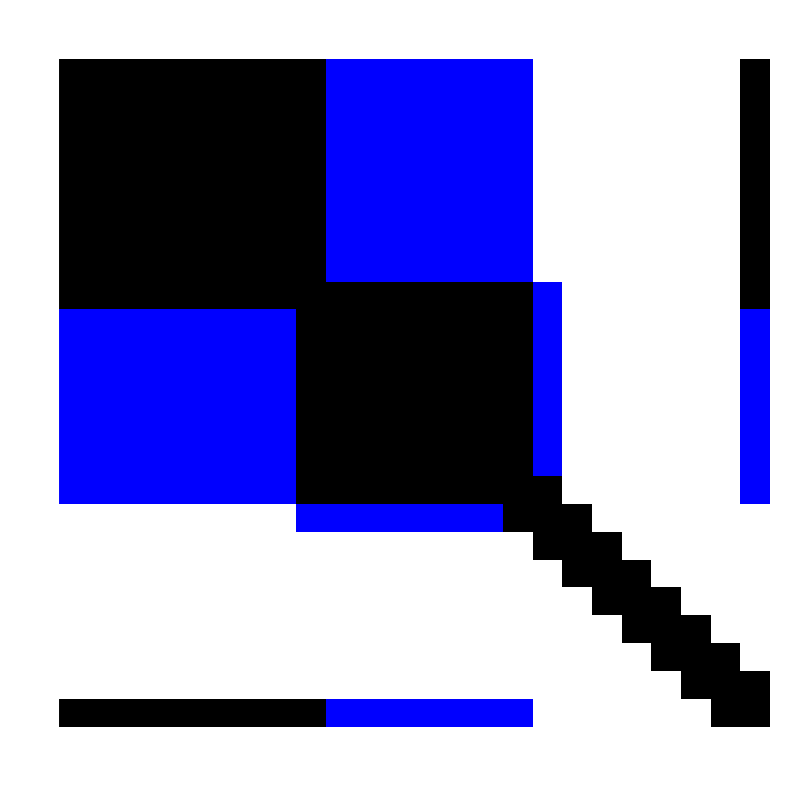
\includegraphics[scale = 0.1]{../figures/fig2_02bm.png}}
&
\raisebox{-.5\height}{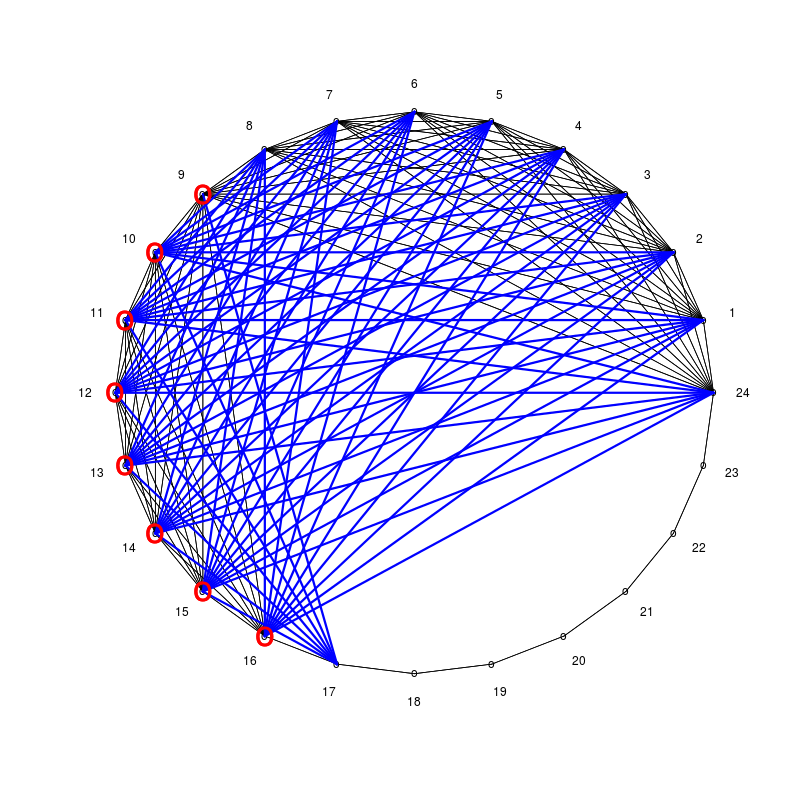
\includegraphics[scale = 0.3]{../figures/fig2_02b.png}}
\end{tabular}
\end{frame}

\begin{frame}
\frametitle{Block APSP}
Iteration 2C: Update all paths
\begin{tabular}{cc}
\raisebox{-.5\height}{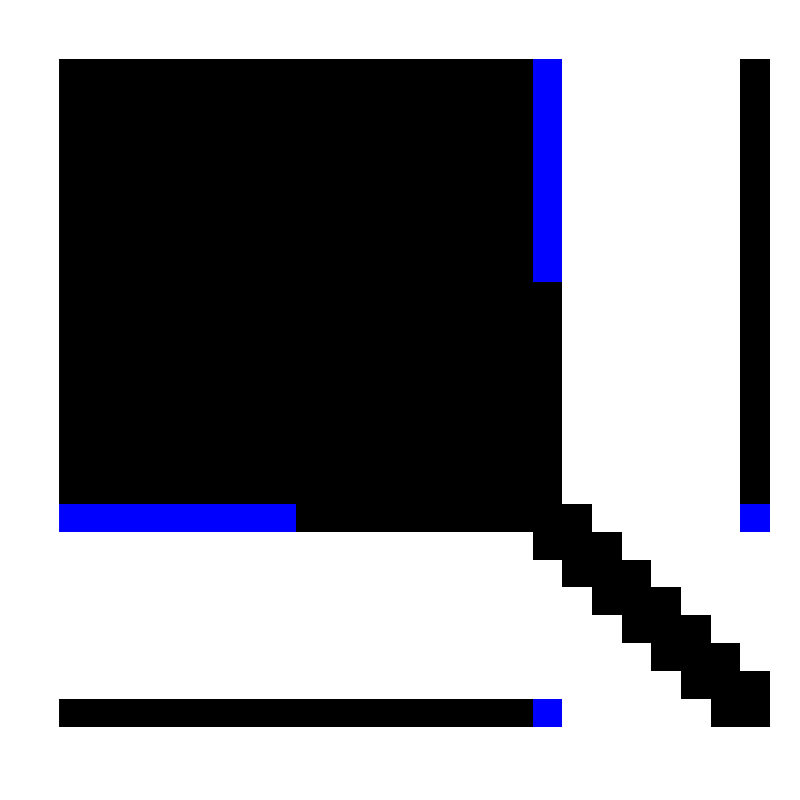
\includegraphics[scale = 0.1]{../figures/fig2_02cm.png}}
&
\raisebox{-.5\height}{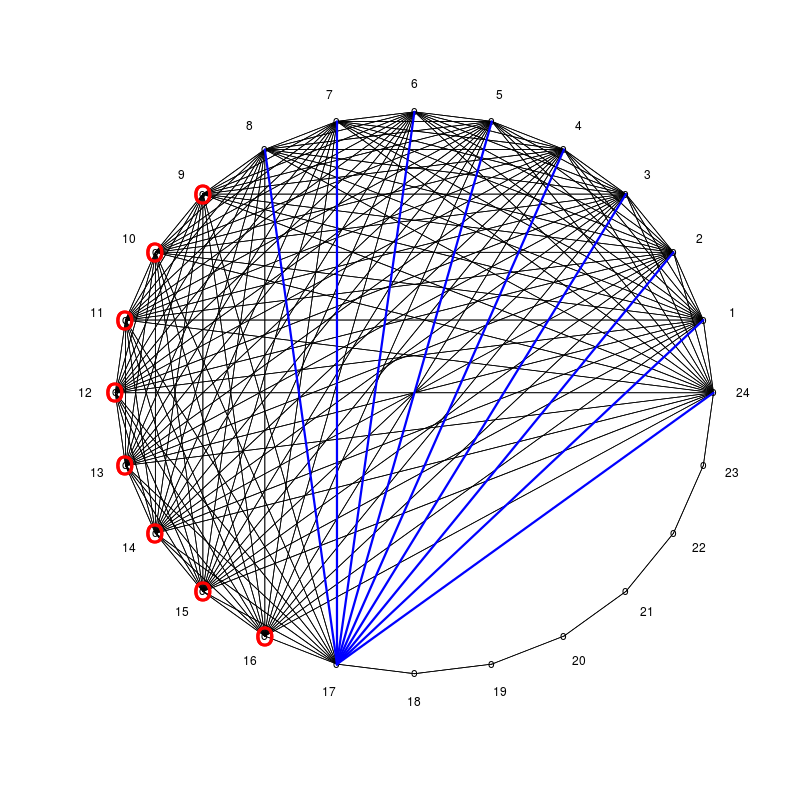
\includegraphics[scale = 0.3]{../figures/fig2_02c.png}}
\end{tabular}
\end{frame}


\begin{frame}
\frametitle{Block APSP}
Iteration 3A: Update all paths within block 3 (with FW)
\begin{tabular}{cc}
\raisebox{-.5\height}{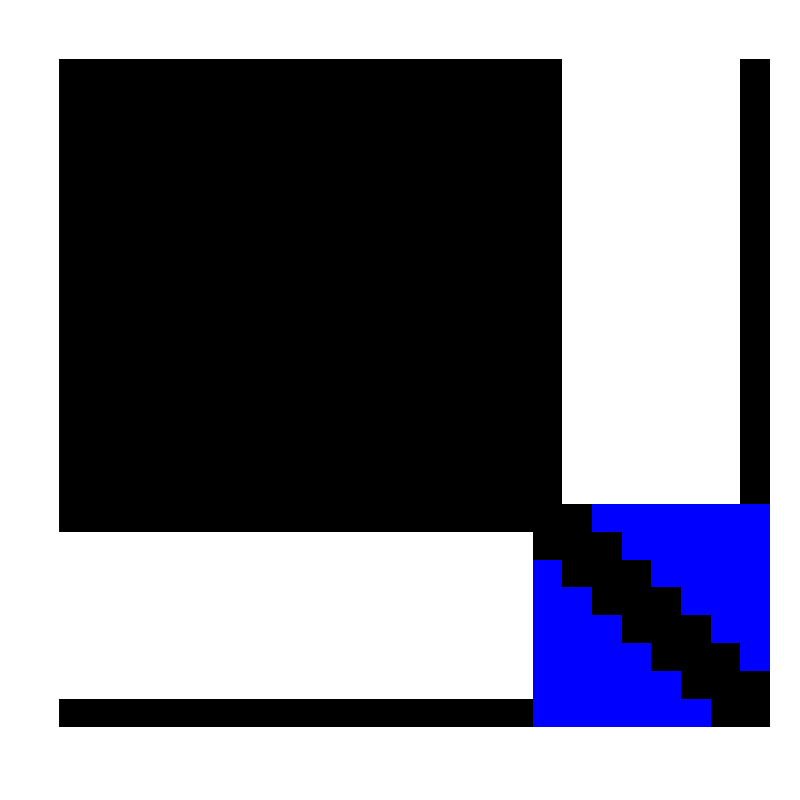
\includegraphics[scale = 0.1]{../figures/fig2_03am.png}}
&
\raisebox{-.5\height}{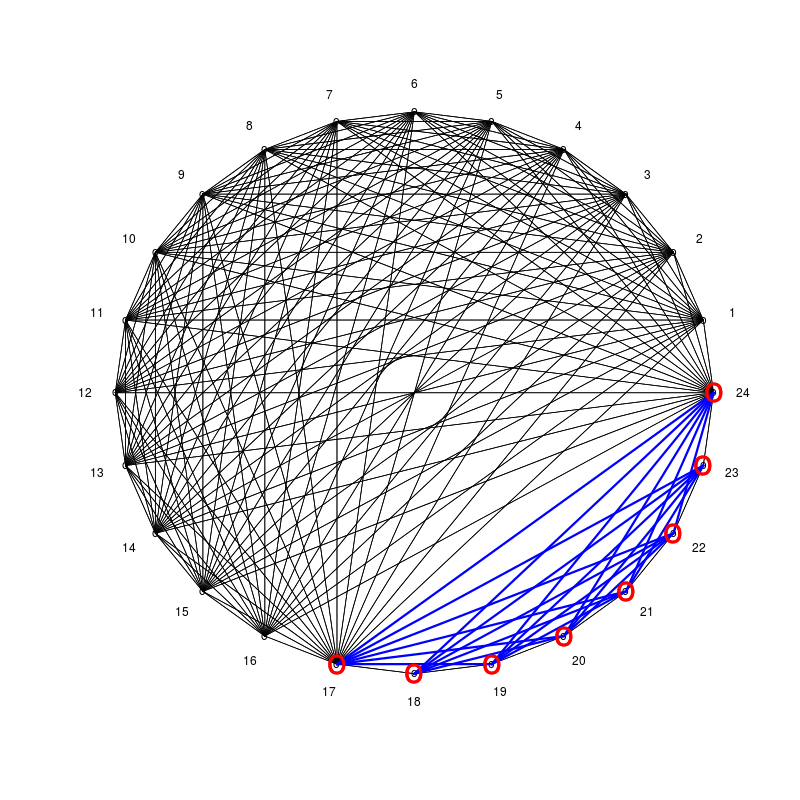
\includegraphics[scale = 0.3]{../figures/fig2_03a.png}}
\end{tabular}
\end{frame}

\begin{frame}
\frametitle{Block APSP}
Iteration 3B: Update all paths to/from block 3
\begin{tabular}{cc}
\raisebox{-.5\height}{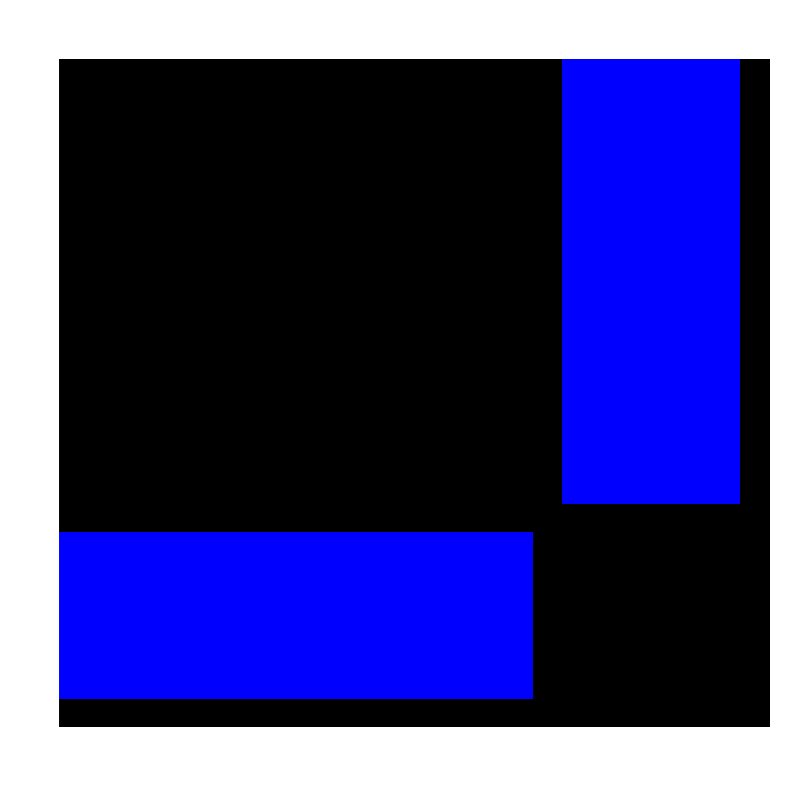
\includegraphics[scale = 0.1]{../figures/fig2_03bm.png}}
&
\raisebox{-.5\height}{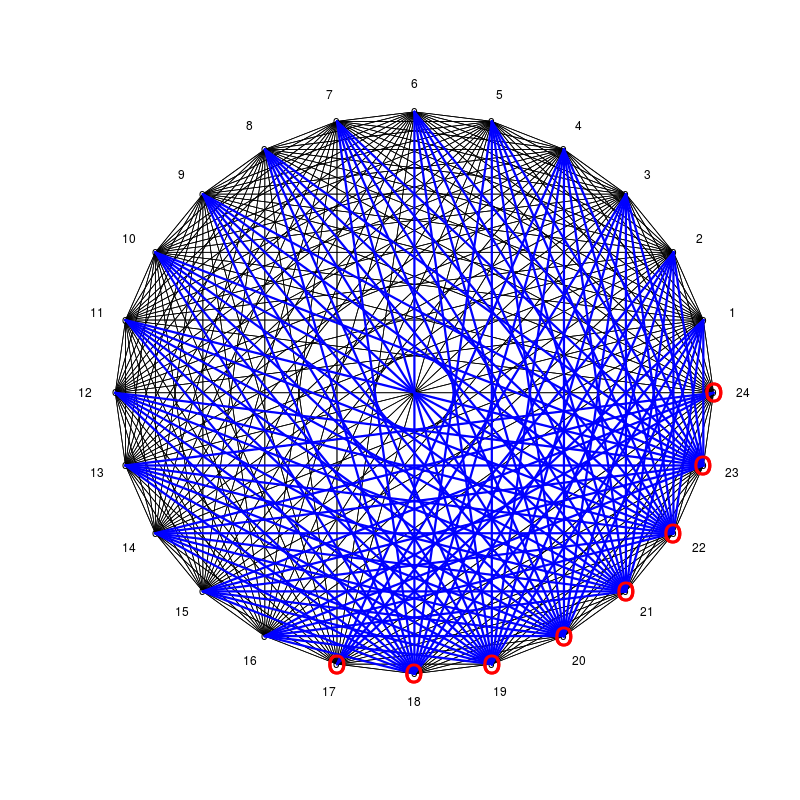
\includegraphics[scale = 0.3]{../figures/fig2_03b.png}}
\end{tabular}
\end{frame}

\begin{frame}
\frametitle{Block APSP}
Iteration 3C: Update all paths, \emph{(terminate)}
\begin{tabular}{cc}
\raisebox{-.5\height}{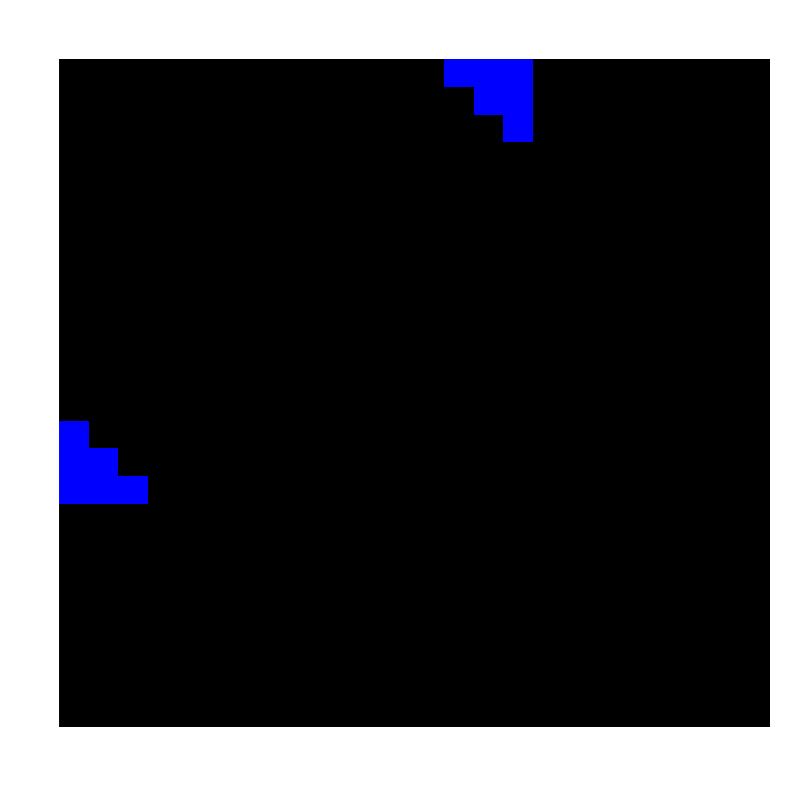
\includegraphics[scale = 0.1]{../figures/fig2_03cm.png}}
&
\raisebox{-.5\height}{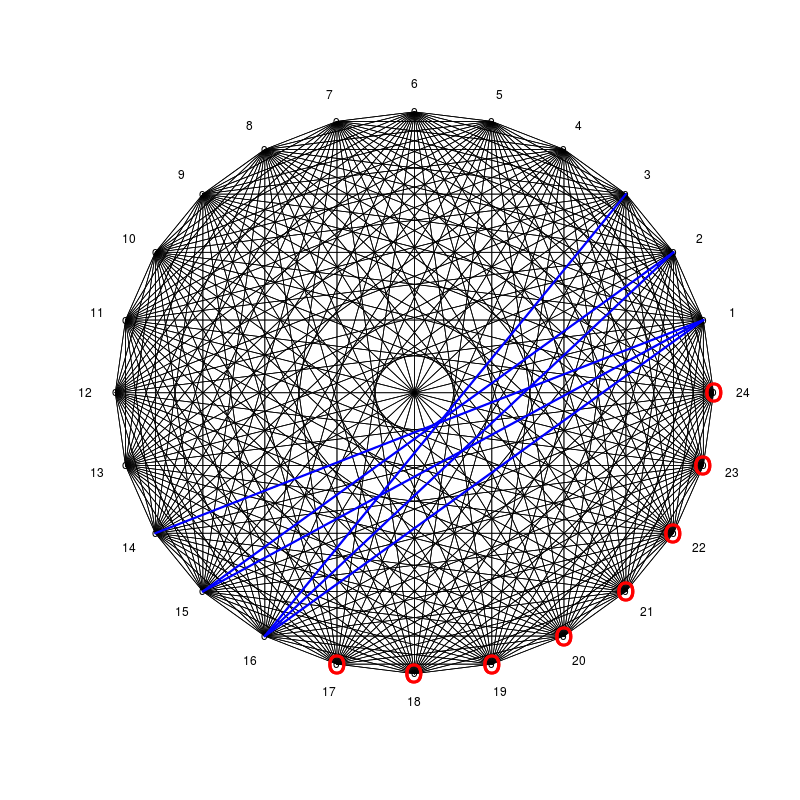
\includegraphics[scale = 0.3]{../figures/fig2_03c.png}}
\end{tabular}
\end{frame}

\begin{frame}
\frametitle{Block APSP: Single-core}
\begin{itemize}
\item Block size $b$, $n/b$ iterations 
\item A-step (all paths within block): $O(b^3)$
\item B-step (all paths to/from block): $O(nb^2)$
\item C-step (all paths): $O(n^2b)$
\item Iteration: $O(n^2 b + nb^2 + b^3)$
\item Total: $O(\frac{n}{b} (n^2 b + nb^2 + b^3)) = O(n^3 + n^2 b + nb^2)$
\item The case $b = 1$ is almost the same as Floyd-Warshall
\end{itemize}
\end{frame}

\begin{frame}
\frametitle{Distributing Block APSP}
\emph{Problem setup}
\begin{itemize}
\item Input format: Given by \emph{dense} adjacency matrix, stored as {\tt BlockMatrix} $S$ with block size $b$
\item Output format: same
\item Let $S[i, j]$ denote the $i, j$th block of $S$
\item Each worker holds $k$ contiguous blocks
\item Set block size $b$ so that $k\frac{n^2}{b^2}$ fits in memory
\end{itemize}
\emph{Scaling}
\begin{itemize}
\item Number of vertices $n \to \infty$
\item Number of workers $p = C_w n^2$
\item Block size $b$, blocks per worker $k$ are constant
\end{itemize}
\end{frame}

\begin{frame}
\frametitle{Distributing Block APSP}
For $i = 1,\hdots, n/b$
\begin{itemize}
\item A-step: \emph{(update all paths within block)}
\begin{itemize}
\item {\tt filter} + {\tt collect} diagonal submatrix $S[i, i]$
\item Driver computes $X = \text{Floyd-Warshall}(S)$ locally
\item Communication cost: $O(b^2)$
\end{itemize} 
\item B-step: \emph{(update all paths to/from block)}
\begin{itemize}
\item {\tt filter} + {\tt mapValues}: update $b$ rows and columns using $X$
\item One-to-all communication (broadcast $X$)
\item Communication cost: $O(b^2 \log(p))$
\end{itemize}
\item C-step: \emph{(update all paths)}
\begin{itemize}
\item {\tt flatMap} to duplicate $b$ rows/columns and {\tt join} to send updated rows/columns to every block
\item {\tt map} to update each block with updated rows/columns
\item All-to-all communication (join)
\item Communication cost: $O(kb^2 p \log p)$
\end{itemize}
\end{itemize}
\end{frame}

\begin{frame}
\frametitle{Distributing Block APSP}
Overall cost:
\begin{itemize}
\item Total computational cost is $O(n^3)$, divided evenly among workers
\item Total communication cost: $O(nb(kp  + 1)\log p)$
\item Total latency/synchronization cost: $O(\frac{n}{b} \log(p))$
\end{itemize}
Optimal performance when $b$ is as large as possible, e.g.
\[
b = \sqrt{\frac{\text{RAM}}{3}}
\]
Hence should be much better than Floyd-Warshall ($b = 1$)
\end{frame}

\begin{frame}
\frametitle{Results}
\end{frame}


\end{document}
